\documentclass[ignorenonframetext,8pt,aspectratio=169]{beamer}

\usepackage{umut}
\usepackage{umuttr}
\usepackage{usynsem}
\usepackage[utf8]{inputenc}
\usepackage{uling}
\usepackage{natbib,unatbib}
\usepackage{linguex}
         \renewcommand{\refdash}{}
\usepackage{ubeamer}
\usepackage{verbatim}
\usepackage{adjustbox}
\usepackage{fancyvrb}

\usepackage{tikz-qtree}
\usetikzlibrary{er,positioning}

\title{VP-internal Subject Hypothesis}
\author{\  \\  {\it Based on Koeneman \& Zeiljstra (2017)} \\ \vspace{20pt} Umut \"Ozge\\  }

\date{COGS 532: Theoretical Linguistics\\ METU, Informatics}

\begin{document}

\begin{frame}\frametitle{}
\thispagestyle{empty}
\maketitle
\end{frame}

\begin{frame}[t,plain]{Agreement}

An uninterpretable feature \setavm{\[ F$^{(u)}$ \]} must be \alert{c-commanded} by a matching \setavm{\[F\]} in the same finite clause; otherwise the sentence is ungrammatical.

\ex. Mary loves herself.

\begin{center}
{\footnotesize
\adjustbox{valign=t}{
\begin{tikzpicture}
\tikzset{level distance=30pt, sibling distance=20pt}
\tikzset{every tree node/.style={align=center,anchor=north}}
				\Tree
				[.{FinP}
					[.{DP} Mary\\{\begin{avm} \[cat  & n \\ det & + \\ $\phi$  & 3, sg\ \\ finite$^{(u)}$ & + \]  \end{avm}} ]
					[.{Fin'} 
						[.{Fin} -s\\{\begin{avm} \[cat  & fin \\ finite  & + \\ $\phi^{(u)}$  & 3, sg\] \end{avm}} ] 
								[.{VP}
								[.{V} love\\{\begin{avm} \[cat  & v \\ \] \end{avm}} ] 
[.{DP} herself\\{\begin{avm} \[cat  & n \\ det & + \\ $\phi^{(u)}$  & 3, sg \\ cat$^{(u)}$ & v \] \end{avm}} ] 
							]
					]
				]
\end{tikzpicture}}
}
\end{center}
\end{frame}

\begin{frame}[t,plain]{VP-internal Subject Hypothesis}
\ex. Mary loves herself.

\begin{center}
{\footnotesize
\adjustbox{valign=t}{
\begin{tikzpicture}
\tikzset{level distance=30pt, sibling distance=20pt}
\tikzset{every tree node/.style={align=center,anchor=north}}
				\Tree
				[.{FinP}
					[.{DP} Mary\\{\begin{avm} \[cat  & n \\ det & + \\ $\phi$  & 3, sg\ \\ finite$^{(u)}$ & + \]  \end{avm}} ]
					[.{Fin'} 
						[.{Fin} -s\\{\begin{avm} \[cat  & fin \\ finite  & + \\ $\phi^{(u)}$  & 3, sg\] \end{avm}} ] 
								[.{VP}
								[.{<DP>} Mary\\{\begin{avm} \[cat  & n \\ det & + \\ $\phi$  & 3, sg\ \\ finite$^{(u)}$ & + \]  \end{avm}} ]
								[.{V'} [.{V} love\\{\begin{avm} \[cat  & v \\ \] \end{avm}} ] 
[.{DP} herself\\{\begin{avm} \[cat  & n \\ det & + \\ $\phi^{(u)}$  & 3, sg \\ cat$^{(u)}$ & v \] \end{avm}} ] 
		] ]
					]
				]
\end{tikzpicture}}
}
\end{center}
\end{frame}

\begin{frame}[t,plain]{Argument 1: {\it There}-constructions}
\ex. \a. There is a man walking in the street.\medskip
\b. A man is walking in the street.

\begin{center}
\begin{tikzpicture}
\tikzset{level distance=30pt, sibling distance=20pt}
\tikzset{every tree node/.style={align=center,anchor=north}}
\Tree[.{FinP} [.{DP} There ] [.{Fin'} [.{Fin} is ] [.{VP} [.{DP} {a man} ] [.{V'} [.{V} walking ] [.{PP} {in the street} ] ] ] ] ] 
\end{tikzpicture}
\end{center}
\end{frame}

\begin{frame}[t,plain]{Argument 2: Floating quantifiers}
\bigskip

		\ex. 
		\a. All the teachers are dancing on the table.
		\b. The teachers are all dancing on the table.
		\b. *The teachers are all dancing on the table.

\bigskip

		\ex.\a. ?Wildly the teachers are dancing on the table.
		\b. The teachers are wildly dancing on the table.
		\b. The teachers are  dancing wildly on the table.

\bigskip

		\ex. \a. Who was dancing on the table? All the teachers.
		\b. Who was dancing on the table? *Wildly the teachers.

\end{frame}

\begin{frame}[t,plain]{Argument 2: Floating quantifiers (cont.)}

\bigskip

\ex.All the teachers.

\begin{center}
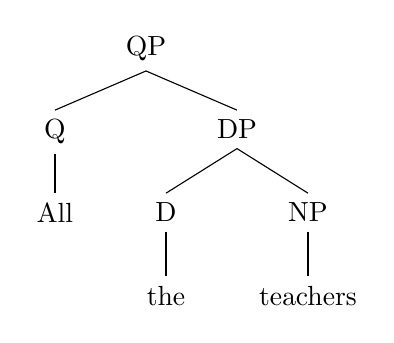
\begin{tikzpicture}
\tikzset{level distance=30pt, sibling distance=20pt}
\tikzset{every tree node/.style={align=center,anchor=north}}
		\Tree [.{QP}
				[.Q All ]
				[.{DP}
					[.{D} the ]
					[.{NP} teachers ] ] ]
\end{tikzpicture}
\end{center}
\end{frame}

\begin{frame}[t,plain]{Argument 2: Floating quantifiers (cont.)}

\vspace{90pt}
\begin{center}

{\small

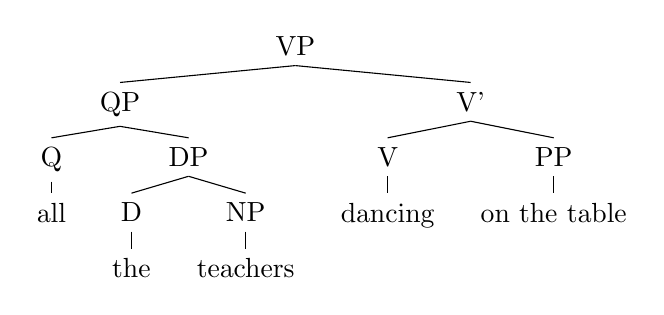
\begin{tikzpicture}
\tikzset{level distance=20pt, sibling distance=10pt}
\tikzset{every tree node/.style={align=center,anchor=north}}
\Tree[.{VP} [.{QP} [.{Q} all ] [.{DP} [.{D} the ] [.{NP} teachers ] ] ] [.{V'} [.{V} dancing ] [.{PP} {on the table} ] ] ] 
\end{tikzpicture}}
		\end{center}
\end{frame}

\begin{frame}[t,plain]{Argument 2: Floating quantifiers (cont.)}

\vspace{90pt}
\begin{center}

{\small

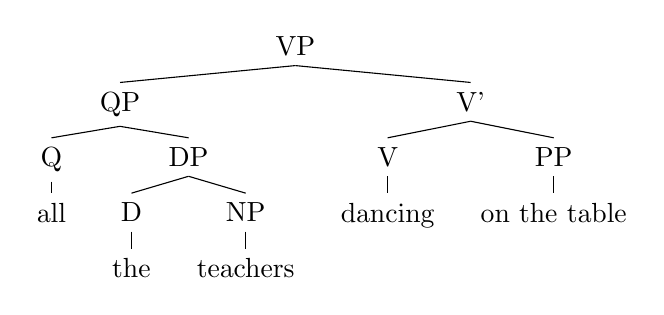
\begin{tikzpicture}
\tikzset{level distance=20pt, sibling distance=10pt}
\tikzset{every tree node/.style={align=center,anchor=north}}
\Tree[.{VP} [.{QP} [.{Q} all ] [.{DP} [.{D} the ] [.{NP} teachers ] ] ] [.{V'} [.{V} dancing ] [.{PP} {on the table} ] ] ] 
\end{tikzpicture}}
		\end{center}

\end{frame}

\begin{frame}[t,plain]{Argument 2: Floating quantifiers (cont.)}

		\ex. (All) the teachers (all) seem (all) to (all) dance (*all) on the table.

\begin{center}
{\footnotesize
\begin{tikzpicture}
\tikzset{level distance=20pt, sibling distance=15pt}
\tikzset{every tree node/.style={align=center,anchor=north}}
		\Tree[.{FinP} [.{}  ] [.{Fin'} [.{Fin} -s ] [.{VP} {}  [.{V'} [.{V} \alert{seem} ] [.{FinP} {}   [.{Fin'} [.{Fin} to ] [.{VP} [.{\colb{QP}} [.{Q} all  ] [.{DP} {the teachers} ] ]
		[.{V'} [.{V} dance ] [.{PP} {on the table} ] ] ] ] ] ] ] ] ]
\end{tikzpicture}}
\end{center}
\end{frame}

\begin{frame}[t,plain]{Argument 3: Idioms}
\ex.\a. \paradigm{\text{John} \\ \text{The baker} \\ \text{Three of his uncles}} \alert{kicked the bucket}.  
\b. \paradigm{\text{John} \\ \text{The baker} \\ \text{Three of his uncles}} \alert{hit the nail on the head}.  
\b. \paradigm{\text{John} \\ \text{The baker} \\ \text{Three of his uncles}} \alert{had cold feet}.  

\bigskip

\ex. \alert{The shadow hit} DP. 

\end{frame}

\begin{frame}[t,plain]{Argument 3: Idioms (cont.)}

\vspace{40pt}

\colb{Idiom principle:}

Only fixed constituents can receive an idiomatic interpretation.

\end{frame}

\begin{frame}[t,plain]{Argument 3: Idioms (cont.)}

\ex. \a. The shit hit the fan.
\b. All hell broke loose.

\bigskip

\ex. The shit \paradigm{\text{has} \\ \text{will} \\ \text{must} } hit the fan.

\vspace{70pt}

\ex. \a. Curiosity killed the cat.
\b. Elvis has left the building.

\end{frame}

\begin{frame}[t,plain]{Argument 4: $\Theta$-role assignment}
\bigskip

\begin{center}
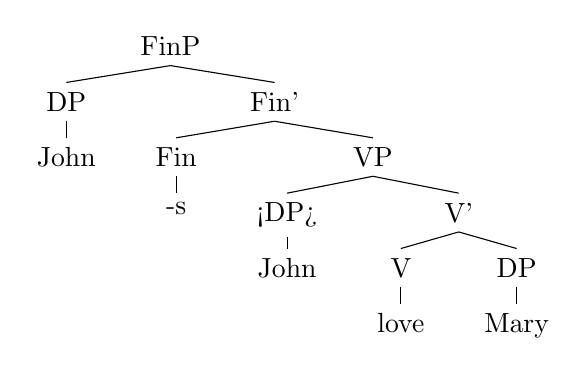
\begin{tikzpicture}
\tikzset{level distance=20pt, sibling distance=15pt}
\tikzset{every tree node/.style={align=center,anchor=north}}
\Tree[.{FinP} [.{DP} John ] [.{Fin'} [.{Fin} -s ] [.{VP} [.{<DP>} John ] [.{V'} [.{V} love ] [.{DP} Mary ] ] ] ] ] 
\end{tikzpicture}
\end{center}
\end{frame}

\end{document}

